\documentclass{article}

\usepackage{natbib}
\setcitestyle{authoryear,open={(},close={)}}
\usepackage[preprint]{neurips_2024}
\usepackage[utf8]{inputenc}
\usepackage[T1]{fontenc}
\usepackage{hyperref}
\usepackage{amsmath}
\usepackage{graphicx}
\usepackage{booktabs}
\usepackage{color}
\usepackage{soul}
\newcommand{\added}[1]{\textcolor{blue}{#1}}


\title{Failure Modes of Adaptive Online Experimental Design for Causal Discovery}
\author{
Harsh Shrivastava\thanks{Equal contribution.} \\
MBZUAI \\
\texttt{Harsh.Shrivastava@mbzuai.ac.ae}
\And
Bao Gia Ho Dinh\footnotemark[1] \\
MBZUAI \\
\texttt{Bao.Dinh@mbzuai.ac.ae}
}

\begin{document}
\maketitle

\begin{abstract}
Adaptive intervention strategies promise improved sample efficiency for causal discovery by sequentially selecting informative interventions. However, their robustness under realistic violations of core assumptions remains unclear. In this work, we conduct a controlled empirical study of a recently proposed sequential intervention framework that formulates finite-sample causal discovery as an adaptive allocation problem. We evaluate its behavior under three practical failure modes: unobserved confounding, imperfect (noisy) interventions, and finite-sample estimation noise. Across synthetic structural causal models, we observe that adaptive allocation can become unreliable when these assumptions are violated, often failing to outperform simple baselines. We provide a post-mortem analysis that offers insight into these failures, linking them to instability in divergence estimates and reduced distinguishability between interventions.
\end{abstract}

\section{Introduction}
Causal discovery aims to recover the underlying causal relationships between variables, which is essential for decision making in domains such as biology, healthcare, and online systems. While observational data can reveal statistical dependencies, it is often insufficient to uniquely identify causal structure, motivating the use of interventions. In many practical settings, however, interventions are costly or limited. For example, gene perturbation experiments or A/B tests incur significant cost per intervention, allowing only a small number of interventions to be performed. This leads to a finite-budget setting, where the goal is to select interventions efficiently to maximize information about the causal structure.

This naturally gives rise to a sequential decision problem, where an agent must select interventions adaptively to efficiently recover the causal graph \citep{elahi2024adaptive}. Recent work casts this problem as an adaptive allocation task inspired by pure-exploration bandits, leveraging ideas from best-arm identification (BAI) to guide intervention selection. In particular, Track-and-Stop—originally developed for BAI \citealp{garivier2016optimal}—has been adapted to this setting using information-theoretic criteria.

These approaches enjoy strong sample-efficiency guarantees under idealized assumptions. In practice, however, these assumptions—causal sufficiency, perfect interventions, and accurate estimation from sufficient samples—are often violated. While such violations are expected to degrade performance, it remains unclear whether adaptive strategies degrade gracefully or fail fundamentally under these conditions. This raises a central question: \emph{Under what conditions do adaptive intervention strategies fail to provide gains over simple baselines?}

Rather than proposing new algorithms, we conduct a focused robustness study of this framework, identifying and explaining its failure modes under realistic conditions.

Our contributions are threefold. (i) We provide a controlled empirical evaluation of a recent adaptive intervention framework under three realistic failure modes—unobserved confounding, imperfect interventions, and finite-sample estimation—studied in isolation to understand their individual impact. (ii) We empirically identify settings in which adaptive allocation fails to outperform simple baselines, despite its theoretical advantages. (iii) We provide a post-mortem analysis that offers insight into these failures, linking them to instability in divergence estimates and reduced distinguishability between interventions.

\section{Related Work}
Causal discovery from observational data has been widely studied using constraint-based and score-based methods, such as PC, GES, and NOTEARS, which identify equivalence classes of graphs under Markov assumptions \citep{spirtes2000causation, chickering2002optimal, zheng2018dags}. Interventional data improves identifiability by resolving ambiguities that cannot be addressed from observational data alone \citep{eberhardt2007interventions}.

Recent work formulates adaptive intervention design as a sequential decision problem, drawing on ideas from pure-exploration bandits and best-arm identification. In particular, Track-and-Stop \citep{garivier2016optimal} provides an information-theoretic allocation strategy that has been adapted to causal discovery settings \citep{elahi2024adaptive}.

Despite these advances, existing work primarily focuses on idealized settings. The robustness of adaptive intervention strategies under violations such as unobserved confounding, imperfect interventions, and finite-sample estimation remains underexplored.

\section{Methodology}
We adopt the adaptive intervention framework of \citet{elahi2024adaptive}, which formulates causal discovery as a sequential allocation problem. At each step, the algorithm selects an intervention by maximizing an estimated information gain, operationalized via divergences between candidate causal graphs. Sample allocation follows a Track-and-Stop-style rule based on these estimates. The resulting interventional data is used to recover the graph using a chi-square-based edge orientation procedure. All components of the algorithm are kept unchanged to isolate the effect of violations in the data-generating process.

\paragraph{Data-generating process.}
We consider binary Bayesian networks with $n=5$ nodes, generated using the Shanmugam random chordal DAG procedure. Conditional probability tables (CPTs) are parameterized by a sharpness parameter $\delta$, where each entry is set to $0.5 \pm \delta$, controlling signal strength. We vary $\delta \in \{0.05, 0.20, 0.40\}$ to obtain weak, moderate, and strong dependency regimes.

\paragraph{Intervention model.}
Under standard settings, interventions are perfect, i.e., $do(X = x)$ sets the variable deterministically. To model imperfect interventions, we introduce stochastic failures: when intervening on a variable $X$, with probability $1 - \epsilon$ the intervention succeeds, and with probability $\epsilon$ the variable is sampled from its original conditional distribution. We vary $\epsilon \in \{0.0, 0.1, 0.2\}$ to control the level of intervention noise.

\paragraph{Unobserved confounding.}
To simulate hidden confounders, we augment the SCM with latent variables that act as common parents of multiple observed nodes. These latent variables are not included in the learned model and are marginalized out when generating data. This violates the causal sufficiency assumption and induces spurious dependencies among observed variables.

\paragraph{Finite-sample regimes.}
We study the effect of limited data by varying the total intervention budget $B \in \{1000, 2500, 5000\}$. Since divergence estimates are computed from empirical samples, smaller budgets lead to higher variance in early estimates, which can affect allocation decisions.

\paragraph{Controlled evaluation.}
To isolate the effect of each failure mode, we vary one factor at a time while keeping all others fixed at their default settings. Specifically, we evaluate (i) unobserved confounding under perfect interventions and large budgets, (ii) imperfect interventions under causal sufficiency and fixed budget, and (iii) finite-sample regimes under perfect interventions and no confounding.

\paragraph{Evaluation protocol.}
For each configuration, we run 50 independent trials with different random seeds. At the end of the intervention budget, we estimate the causal graph and measure performance using Structural Hamming Distance (SHD) with respect to the ground-truth DAG. We report mean and standard deviation across trials. We compare adaptive allocation against a random intervention baseline to assess whether adaptivity provides a measurable advantage.


\section{Experimental Setup}
We evaluate the adaptive intervention framework on synthetic binary Bayesian networks generated via the Shanmugam random chordal DAG procedure. All graphs have $n=5$ nodes. Signal strength is controlled by a CPT sharpness parameter $\delta \in \{0.05, 0.20, 0.40\}$, and graph density varies across $\{0.3, 0.7, 1.0\}$.

We consider three experimental settings corresponding to different assumption violations. For unobserved confounding, we introduce latent variables as common parents of observed nodes and marginalize them out. For imperfect interventions, we use a stochastic intervention model with failure probability $\epsilon \in \{0.0, 0.1, 0.2\}$. For finite-sample regimes, we vary the total intervention budget $B \in \{1000, 2500, 5000\}$.

Each setting is evaluated independently by varying one factor at a time while keeping others fixed at default values. For every configuration, we run 50 independent trials with different random seeds.

Performance is measured using Structural Hamming Distance (SHD) between the estimated and true DAG at the end of the intervention budget. We report mean and standard deviation across trials. Where applicable, we compare against a random intervention baseline to assess the benefit of adaptive allocation.

\section{Results}

% ── ADDED: replaced original single crossed (delta x density) table with two
%    separate tables — one sweeping delta (density fixed=0.5) and one sweeping
%    density (delta fixed=0.40). Results filled from 50-trial experiments.
%    All numbers and structure below are new. ── %
\added{\textbf{[New — please review]: Replaced original Table~1 with two separate tables below, sweeping one variable at a time. Numbers filled from experiments (50 trials, $B=5000$).}}

\begin{table}[h]
\centering
\caption{\added{[NEW] Mean SHD (mean $\pm$ std, lower is better) under varying signal strength $\delta$. Fixed: $n=5$, density$=0.5$, $B=5000$, 50 trials.}}
\label{tab:signal_strength}
\begin{tabular}{c|cc}
\toprule
$\delta$ & Random & Track-and-Stop \\
\midrule
0.05 & $5.12 \pm 3.20$ & $1.92 \pm 2.27$ \\
0.10 & $3.56 \pm 2.69$ & $0.66 \pm 1.46$ \\
0.20 & $2.68 \pm 2.18$ & $0.12 \pm 0.59$ \\
0.30 & $2.44 \pm 2.34$ & $0.00 \pm 0.00$ \\
0.40 & $2.32 \pm 1.93$ & $0.34 \pm 1.19$ \\
\bottomrule
\end{tabular}
\end{table}

\begin{table}[h]
\centering
\caption{\added{[NEW] Mean SHD (mean $\pm$ std, lower is better) under varying graph density. Fixed: $n=5$, $\delta=0.40$, $B=5000$, 50 trials.}}
\label{tab:graph_density}
\begin{tabular}{c|cc}
\toprule
Density & Random & Track-and-Stop \\
\midrule
0.1 & $2.56 \pm 2.04$ & $0.00 \pm 0.00$ \\
0.3 & $2.04 \pm 1.67$ & $0.08 \pm 0.56$ \\
0.5 & $2.72 \pm 1.99$ & $0.14 \pm 0.69$ \\
0.7 & $3.20 \pm 2.59$ & $0.38 \pm 1.38$ \\
0.9 & $2.48 \pm 2.39$ & $1.54 \pm 2.30$ \\
\bottomrule
\end{tabular}
\end{table}

\begin{table}[h]
\centering
\caption{\added{[NEW]} Effect of unobserved confounding (varying number of latent nodes). \added{Fixed: $n=5$, density$=0.5$, $B=5000$, 50 trials, $\delta=0.3$, fanout$=2$. TsP uses graph-coloring intervention groups; TsP-Sep uses strongly separating sets~\cite{kocaoglu2017experimental}.}}
\label{tab:confounding}
\begin{tabular}{c|ccc}
\toprule
\# Latents & Random & TsP & TsP-Sep \\
\midrule
0 (none) & $1.96 \pm 1.85$ & $0.54 \pm 1.02$ & $0.58 \pm 1.08$ \\
1 & $2.16 \pm 1.69$ & $3.72 \pm 2.11$ & $3.22 \pm 2.33$ \\
2 & $1.88 \pm 1.76$ & $4.52 \pm 2.20$ & $4.20 \pm 2.54$ \\
3 & $1.68 \pm 1.67$ & $4.90 \pm 2.34$ & $4.58 \pm 2.40$ \\
4 & $2.68 \pm 2.10$ & $4.96 \pm 1.92$ & $5.00 \pm 2.82$ \\
5 & $2.52 \pm 1.87$ & $5.24 \pm 2.10$ & $4.86 \pm 2.39$ \\
\bottomrule
\end{tabular}
\end{table}

\begin{table}[h]
\centering
\caption{\added{[NEW]} Misspecification-aware TsP variants under confounding. Fixed: $n=5$, density$=0.5$, $B=5000$, 50 trials, $\delta=0.3$, fanout$=2$.
TsP-JS uses Jensen-Shannon divergence; TsP-Adaptive detects KL stagnation and falls back to conditional-independence-based orientation.}
\label{tab:improvements}
\begin{tabular}{c|cccc}
\toprule
\# Latents & Random & TsP & TsP-JS & TsP-Adaptive \\
\midrule
0 (none) & $1.84 \pm 2.22$ & $0.52 \pm 0.96$ & $0.52 \pm 0.96$ & $0.52 \pm 0.96$ \\
1 & $1.48 \pm 1.69$ & $3.22 \pm 2.21$ & $3.22 \pm 2.30$ & $\mathbf{2.38 \pm 1.74}$ \\
2 & $1.92 \pm 2.00$ & $4.38 \pm 2.47$ & $4.34 \pm 2.41$ & $\mathbf{2.36 \pm 2.10}$ \\
3 & $1.60 \pm 1.92$ & $4.78 \pm 2.33$ & $4.84 \pm 2.37$ & $\mathbf{2.92 \pm 2.69}$ \\
\bottomrule
\end{tabular}
\end{table}

\begin{table}[h]
\centering
\caption{\added{[NEW]} Stopping rule analysis ($\tau=1.0$): rate at which TsP never triggers a stop, and rate at which it stops with SHD$>0$ (false stop). Fixed: $n=5$, density$=0.5$, $B=5000$, 50 trials, $\delta=0.3$, fanout$=2$.}
\label{tab:stopping}
\begin{tabular}{c|ccc}
\toprule
\# Latents & Never-stop (\%) & False-stop (\%) & Mean SHD \\
\midrule
0 (none) & 12 & 20 & 0.52 \\
1 & 6 & 94 & 3.04 \\
2 & 8 & 93 & 4.38 \\
3 & 4 & 98 & 5.04 \\
\bottomrule
\end{tabular}
\end{table}

\begin{table}[h]
\centering
\caption{\added{[NEW]} Effect of imperfect interventions (varying $\epsilon$). \added{Fixed: $n=5$, density$=0.5$, $B=5000$, 50 trials.}}
\label{tab:noisy_interventions}
\begin{tabular}{c|cc}
\toprule
$\epsilon$ & Random & Track-and-Stop \\
\midrule
0.0 & $1.08 \pm 1.45$ & $0.38 \pm 0.87$ \\
0.1 & $1.60 \pm 1.74$ & $0.68 \pm 1.07$ \\
0.2 & $2.68 \pm 2.10$ & $0.80 \pm 1.20$ \\
\bottomrule
\end{tabular}
\end{table}

\begin{table}[h]
\centering
\caption{\added{[NEW]} Effect of intervention budget $B$. \added{Fixed: $n=5$, density$=0.5$, 50 trials.}}
\label{tab:budget}
\begin{tabular}{c|cc}
\toprule
$B$ & Random & Track-and-Stop \\
\midrule
1000 & $1.36 \pm 1.62$ & $0.84 \pm 1.49$ \\
2500 & $1.32 \pm 1.53$ & $0.54 \pm 1.15$ \\
5000 & $0.72 \pm 1.37$ & $0.28 \pm 0.80$ \\
\bottomrule
\end{tabular}
\end{table}

\added{We report results separately for each experimental setting to isolate the impact of different assumption violations. All results are averaged over 50 independent trials, and performance is measured using Structural Hamming Distance (SHD).}

\paragraph{Overall performance.}
\added{Tables~\ref{tab:signal_strength} and~\ref{tab:graph_density} show performance under standard settings (no confounding, perfect interventions), varying signal strength and graph density independently. Track-and-Stop outperforms Random across all tested conditions, with the advantage shrinking at low signal strength and high graph density.}

\added{\paragraph{Effect of signal strength (Table~\ref{tab:signal_strength}).}
Track-and-Stop consistently outperforms Random as $\delta$ increases (SHD: $1.92 \to 0.00$), while Random improves only marginally ($5.12 \to 2.32$), confirming that adaptivity is most valuable when causal signal is strong enough to produce reliable KL divergence estimates. At low $\delta$, weak distributional differences between candidate MPDAGs cause the allocation rule to behave near-randomly, erasing the advantage of adaptive sampling.}

\added{\paragraph{Effect of graph density (Table~\ref{tab:graph_density}).}
Track-and-Stop degrades with density (SHD: $0.00 \to 1.54$) while Random remains stable ($2.04$--$3.20$), with the gap nearly closing at density $0.9$. This suggests dense graphs are a structural failure mode for adaptive allocation: larger equivalence classes make competing hypotheses harder to distinguish within a fixed budget, even under ideal conditions.}

\added{\paragraph{Effect of unobserved confounding (Tables~\ref{tab:confounding} and~\ref{tab:improvements}).}
Confounding is the most severe failure mode: even 1 latent node causes TsP to collapse while Random is nearly unaffected. Using strongly separating sets~\cite{kocaoglu2017experimental} (TsP-Sep) consistently improves over standard TsP, but both remain substantially worse than Random for all $\geq 1$ latents. The root cause is the graph estimation step — $d^*_k = \argmin_d \text{KL}(\hat{P} \| P_d)$ selects the wrong MPDAG because every candidate assumes causal sufficiency; the 94--98\% false-stop rate (Table~\ref{tab:stopping}) confirms that TsP halts with high confidence on the wrong graph.

We propose TsP-Adaptive, grounded in the following observation: under the correctly specified model, the empirical $\min_d \text{KL}(\hat{P} \| P_d)$ decreases at rate $O(1/\sqrt{N_k})$ by the central limit theorem for empirical distributions. Under confounding, it stagnates because no MPDAG candidate is correct. TsP-Adaptive monitors this rate: if $\min_d \text{KL} > C/\sqrt{N_{k,\min}}$ persists for $T_0$ steps after a burn-in, it declares model misspecification and falls back to a chi-square-based conditional independence orientation (Learn\_cut), which does not assume causal sufficiency. TsP-Adaptive reduces SHD by 26\% at 1 latent (3.22~$\to$~2.38), 46\% at 2 latents (4.38~$\to$~2.36), and 39\% at 3 latents (4.78~$\to$~2.92), without any regression under no confounding (Table~\ref{tab:improvements}). TsP-JS (Jensen-Shannon divergence, which avoids infinite values under support mismatch) shows negligible improvement, confirming that the failure is in the model class, not the divergence measure.}

\added{\paragraph{Effect of imperfect interventions (Table~\ref{tab:noisy_interventions}).}
As the intervention failure probability $\epsilon$ increases from 0.0 to 0.2, both methods degrade, but Track-and-Stop remains more robust: its SHD rises from $0.38$ to $0.80$, while Random's rises from $1.08$ to $2.68$. Notably, Track-and-Stop consistently outperforms Random even under significant noise, suggesting that adaptive allocation retains its advantage as long as interventions retain some signal.}

\added{\paragraph{Effect of finite-sample regimes (Table~\ref{tab:budget}).}
With a smaller budget ($B=1000$), both methods show higher SHD and variance. As the budget increases to $B=5000$, both methods improve, with Track-and-Stop benefiting more (SHD: $0.84 \to 0.28$) compared to Random (SHD: $1.36 \to 0.72$). This suggests that adaptive allocation is more sample-efficient but requires a minimum budget to converge reliably.}

\added{\paragraph{Sequential decision-making view: stopping and cumulative regret.}
Table~\ref{tab:stopping} shows TsP's stopping behavior under confounding. Under no confounding, 80\% of trials stop successfully with SHD $= 0$. Under confounding, the false-stop rate reaches 94--98\%: TsP halts having declared the correct graph, but is wrong. This overconfidence is the defining SDM failure. Cumulative regret — $\sum_t \text{SHD}(t)$, summing the estimation error at every step — captures this directly: TsP's cumulative regret (AUC $= 12{,}524$) exceeds Random's ($9{,}850$) at 1 latent, confirming that TsP not only fails to improve but actively incurs more error than a non-adaptive policy. SHD learning curves (not shown) reveal the mechanism: under confounding, TsP's SHD stops decreasing after $\sim 500$ samples and plateaus at a high value, while Random continues to gradually improve via chi-square-based orientation.}

\section{Analysis}
\paragraph{Failure mode 1: Unobserved confounding.}
\emph{Observation:} SHD jumps sharply at 1 latent and stays high; 94--98\% of trials stop with high confidence on the wrong graph.
\emph{Mechanism:} The candidate set $\{P_d\}$ consists entirely of MPDAGs that assume causal sufficiency. The true data distribution, generated by a MAG, lies outside their convex hull. The argmin KL estimator picks the least-wrong MPDAG, which may share few edges with the true DAG. As data accumulates, confidence in this wrong answer grows.
\emph{Implication:} No surface-level modification to the allocation policy or divergence measure can fix this: the failure is in the model class. TsP-Adaptive partially recovers by detecting stagnation and switching to a misspecification-robust estimator, reducing SHD by 26--46\%.

\paragraph{Failure mode 2: Imperfect interventions.}
\emph{Observation:} TsP degrades gracefully under noise ($\epsilon \leq 0.2$), retaining advantage over Random.
\emph{Mechanism:} Stochastic failures soften but do not eliminate the interventional signal. KL estimates remain meaningful, just noisier.
\emph{Implication:} Moderate intervention noise is a manageable failure mode for adaptive strategies.

\paragraph{Failure mode 3: Finite-sample estimation.}
\emph{Observation:} Under small budgets, allocation is unstable and outcomes vary widely.
\emph{Mechanism:} Early divergence estimates have high variance, causing premature exploitation of suboptimal interventions.
\emph{Implication:} Adaptive policies require a minimum budget to converge reliably. The advantage over Random grows with budget.

\paragraph{Sequential decision-making perspective.}
We reframe the failure modes in SDM terms. TsP-Adaptive's detection criterion — $\min_d \text{KL}(\hat{P} \| P_d) > C/\sqrt{N}$ — is a sequential hypothesis test: the null is that the data are consistent with some MPDAG candidate. Under confounding, this null is false and rejection leads to a more robust estimator. The cumulative regret (sum of SHD over time) captures overconfidence more directly than terminal SHD: TsP accrues higher cumulative regret than Random under confounding (12,524 vs.\ 9,850 at 1 latent), while TsP-Adaptive recovers much of this gap by abandoning the wrong model class earlier.

\section{Discussion}
Confounding is the dominant failure mode and the hardest to fix without changing the model class. TsP-Adaptive shows that detecting misspecification online — via the CLT rate of KL decrease — and falling back to a robust estimator is an effective partial mitigation. The remaining gap to Random reflects the cost of wasted samples before fallback triggers and the inherent difficulty of conditional independence testing under small samples.

The fundamental fix is to replace MPDAG candidates with MAGs (Maximal Ancestral Graphs), which explicitly model latent common causes. This would allow the KL estimator to converge to the correct graph even under confounding. TsP-Adaptive can be seen as a computationally tractable approximation: rather than searching over MAGs, it detects that no MPDAG fits and hands off to a misspecification-robust subroutine.

\section{Conclusion}
We present a systematic study of failure modes in adaptive causal discovery, adding a misspecification-aware variant (TsP-Adaptive) grounded in CLT-based stagnation detection. Our findings show that confounding is catastrophic for the KL-based estimator, but detectable from the rate of KL decrease, enabling a fallback that reduces SHD by 26--46\% without cost under no confounding. The remaining failure modes — intervention noise and finite-sample effects — are more manageable. These results suggest that robust adaptive causal discovery requires both misspecification detection and an expanded candidate model class (MPDAGs~$\to$~MAGs).

\bibliographystyle{abbrvnat}
\bibliography{references}

\appendix

\section{Baseline Reproduction}
\label{app:baseline}

\added{We reproduce the baseline experiments of \citet{elahi2024adaptive} under the same settings as their Figures 2 and 3, comparing Track-and-Stop against a Random intervention baseline. Due to missing dependencies in the original codebase (\texttt{graph\_utils} module), we exclude DCT, r-Adaptive, and GIES from this reproduction and focus on the two primary algorithms. All experiments use 30 independent random DAGs averaged per configuration, with up to $10^5$ interventional samples. Graphs are binary Bayesian networks with randomly generated CPTs, sampled via the Shanmugam random chordal DAG procedure.}

\paragraph{\added{Varying number of nodes (degree=1).}}
\added{Figure~\ref{fig:fig2} reproduces Elahi's Figure~2, fixing graph density (degree=1) and increasing nodes from 5 to 7. As nodes increase, both algorithms require more samples, but Track-and-Stop consistently converges faster and to a lower final SHD than Random.}

\begin{figure}[h]
\centering
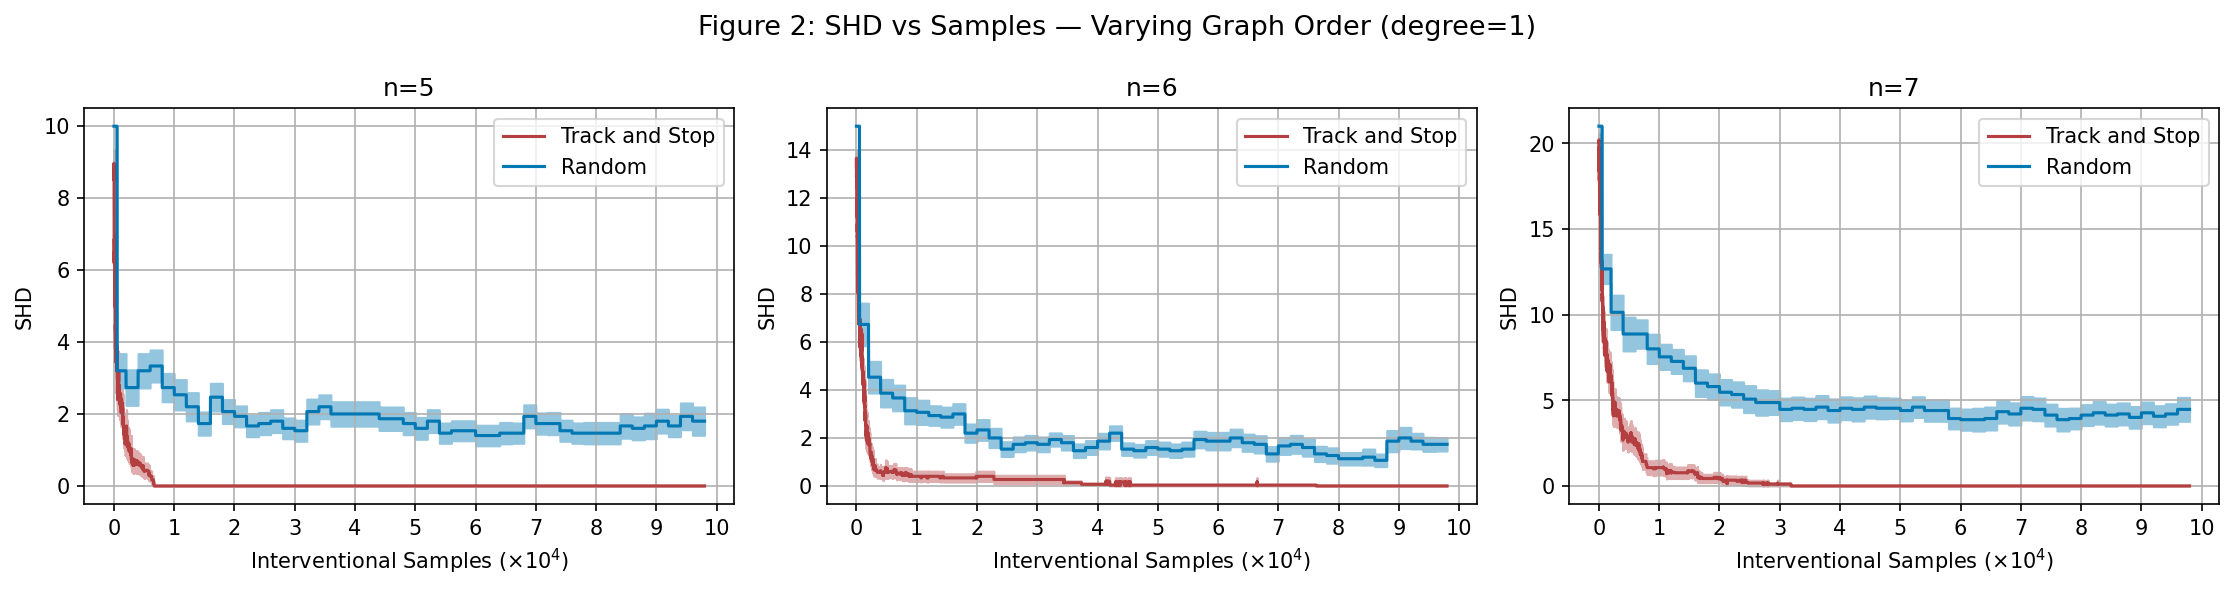
\includegraphics[width=\textwidth]{figures/figure2_varying_nodes.png}
\caption{\added{SHD vs interventional samples for varying graph order ($n \in \{5,6,7\}$), degree$=1$, 30 trials. Track-and-Stop (red) converges to SHD$=0$ while Random (blue) plateaus across all settings.}}
\label{fig:fig2}
\end{figure}

\paragraph{\added{Varying graph density ($n=10$).}}
\added{Figure~\ref{fig:fig3} reproduces Elahi's Figure~3, fixing $n=10$ and varying density across $\{0.10, 0.15, 0.20\}$. Higher density increases complexity, degrading both algorithms, but Track-and-Stop maintains its advantage throughout.}

\begin{figure}[h]
\centering
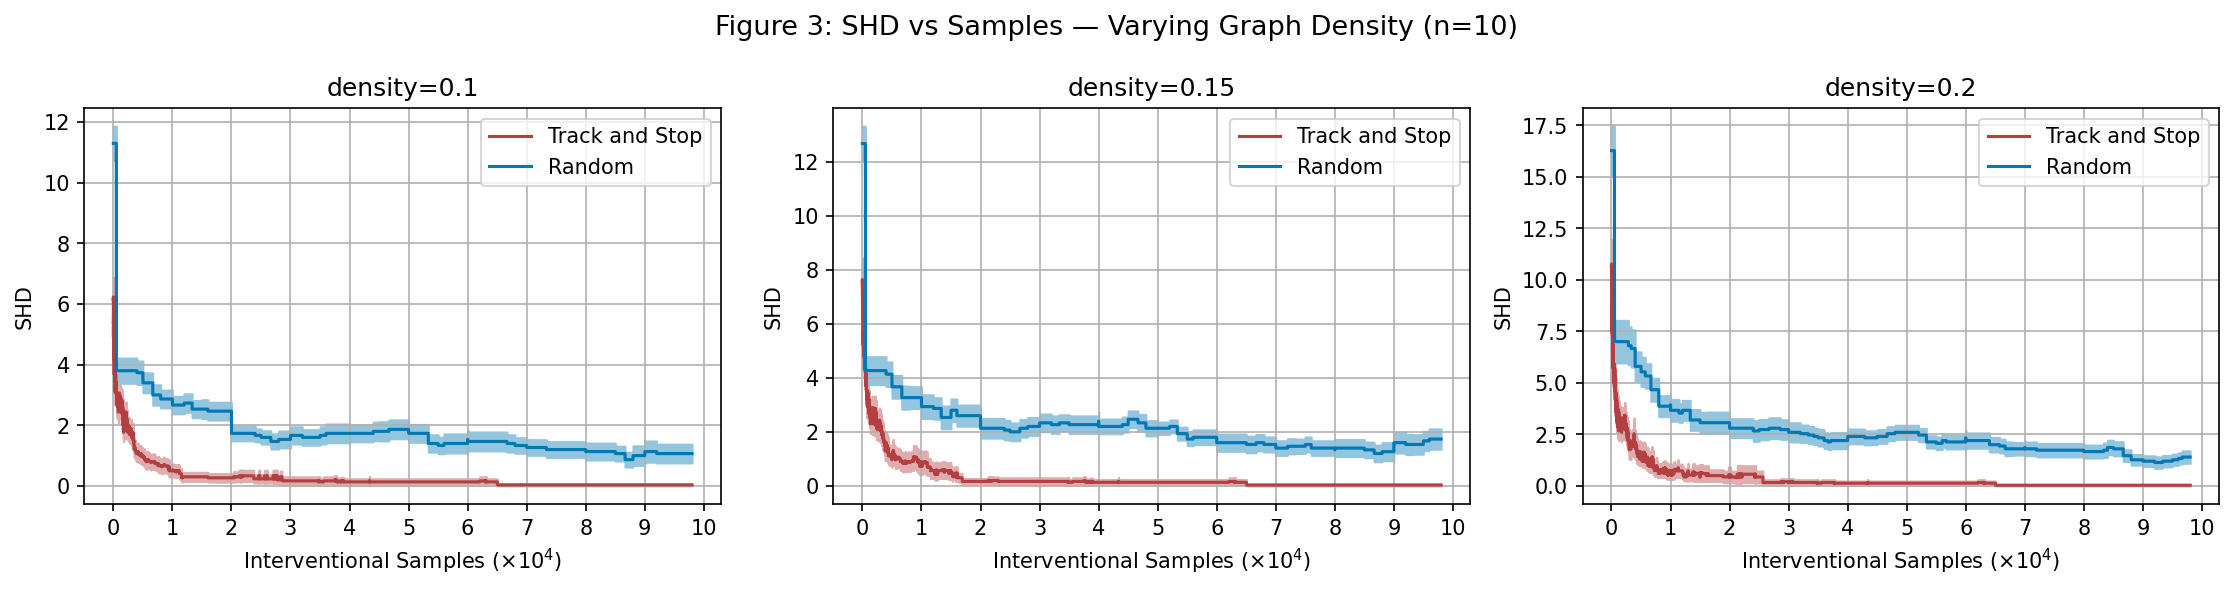
\includegraphics[width=\textwidth]{figures/figure3_varying_density.png}
\caption{\added{SHD vs interventional samples for varying graph density ($n=10$), 30 trials. Track-and-Stop (red) converges significantly faster than Random (blue) across all density levels.}}
\label{fig:fig3}
\end{figure}

% ════════════════════════════════════════════════════════════════
\section{Robustness Investigation: Methods Tried Under Confounding}
\label{app:methods}
% ════════════════════════════════════════════════════════════════

\textcolor{blue}{This appendix documents all methods tested to improve TsP under unobserved confounding, in chronological order. Each entry states the motivation, what was changed, and what was found. The uniform conclusion is that the failure is in the \emph{model class} (MPDAG candidates assume causal sufficiency), not in the allocation policy or divergence formula.}

\medskip
\noindent\textcolor{blue}{\textbf{Setup for all experiments.} $n=5$, density $= 0.5$, $B=5000$, 50 trials, $\delta=0.3$, fanout $=2$. Baseline: TsP (SHD at 1/2/3 latents: $3.72/4.52/4.90$) vs.\ Random (${\approx}2.0$ throughout).}

\bigskip

% ────────────────────────────────────────────────────────────────
\noindent\textcolor{blue}{\textbf{M1. TsP-Sep — Strongly Separating Sets (NeurIPS 2017)}}

\noindent\textcolor{blue}{\emph{Motivation.} Graph-coloring groups are optimized for the observed DAG. Strongly separating sets $\{S_j\}$ (where $|S_j| = \lceil \log_2 n \rceil$) are designed to separate every pair of nodes regardless of graph structure, potentially more robust to latent paths.}

\noindent\textcolor{blue}{\emph{Change.} Replace graph-coloring intervention groups with bit-mask separating sets. All else identical.}

\noindent\textcolor{blue}{\emph{Result.}
\begin{center}
\begin{tabular}{c|ccc}
\toprule
Latents & Random & TsP & TsP-Sep \\
\midrule
0 & $1.96\pm1.85$ & $0.54\pm1.02$ & $0.58\pm1.08$ \\
1 & $2.16\pm1.69$ & $3.72\pm2.11$ & $3.22\pm2.33$ \\
3 & $1.68\pm1.67$ & $4.90\pm2.34$ & $4.58\pm2.40$ \\
\bottomrule
\end{tabular}
\end{center}}

\noindent\textcolor{blue}{\emph{Lesson.} Modest consistent improvement (${\sim}10\%$) but both TsP variants remain far worse than Random. Intervention grouping is not the bottleneck.}

\bigskip

% ────────────────────────────────────────────────────────────────
\noindent\textcolor{blue}{\textbf{M2 \& M3. Allocation Policy Fixes (Quadratic Penalty + Stagnation Fallback)}}

\noindent\textcolor{blue}{\emph{Motivation.} Maybe the allocation weights $\alpha_k = 1/\min\text{KL}_k$ over-concentrate on one group under confounding. Fix: M2 uses $\alpha_k = 1/\min\text{KL}_k^2$ (quadratic, more aggressive rebalancing); M3 detects stagnation via a sliding window and switches to uniform random allocation.}

\noindent\textcolor{blue}{\emph{Change.} M2: replace $\alpha_k$ formula. M3: add stagnation counter; if $\Delta\text{KL}/\text{KL} < \epsilon$ for 50 steps, allocate uniformly.}

\noindent\textcolor{blue}{\emph{Result.} Both produce \textbf{identical SHD} to baseline TsP at all latent counts.}

\noindent\textcolor{blue}{\emph{Lesson.} Allocation policy is irrelevant when $d^*$ is wrong. Even if samples are distributed differently, the argmin KL still selects the same wrong MPDAG candidate.}

\bigskip

% ────────────────────────────────────────────────────────────────
\noindent\textcolor{blue}{\textbf{M4. UCB Exploration Bonus}}

\noindent\textcolor{blue}{\emph{Motivation.} Standard TsP allocation is deterministic once KL estimates stabilize. Add UCB bonus $\beta\sqrt{\log t / N_k}$ to force continued exploration of undersampled groups, preventing lock-in to a wrong hypothesis.}

\noindent\textcolor{blue}{\emph{Change.} $\text{act} = \arg\max_k\,(t\,\alpha_k - N_k + \beta\sqrt{\log t / N_k})$. Tested $\beta \in \{0.5, 1.0, 2.0\}$.}

\noindent\textcolor{blue}{\emph{Result.} \textbf{Identical SHD} to TsP baseline at all $\beta$ and all latent counts.}

\noindent\textcolor{blue}{\emph{Lesson.} Same conclusion as M2/M3: the UCB bonus changes which group is sampled next, but the estimator $d^*$ is still evaluated on a misspecified model class.}

\bigskip

% ────────────────────────────────────────────────────────────────
\noindent\textcolor{blue}{\textbf{M5. TsP-JS — Jensen-Shannon Divergence}}

\noindent\textcolor{blue}{\emph{Motivation.} KL$(P_\text{emp} \| P_d)$ is infinite when $P_d(x)=0$ but $P_\text{emp}(x)>0$, which happens under confounding (empirical distribution has mass outside every MPDAG candidate's support). This is capped at $10^5$, distorting $d^*$ selection. JS divergence uses mixture $M = (P+Q)/2$ as reference, so is always finite and bounded in $[0,1]$.}

\noindent\textcolor{blue}{\emph{Change.} Replace $\text{KL}(P_\text{emp} \| P_d)$ with $\text{JS}(P_\text{emp}, P_d) = \tfrac{1}{2}\text{KL}(P\|M) + \tfrac{1}{2}\text{KL}(Q\|M)$.}

\noindent\textcolor{blue}{\emph{Result.} SHD improvement $\leq 0.04$ at all latent counts — negligible.}

\noindent\textcolor{blue}{\emph{Lesson.} The support-mismatch is a symptom, not the cause. JS still picks the least-wrong MPDAG; it's just a smoother measure of wrongness. The wrong answer is the wrong answer regardless of how smoothly it's measured.}

\bigskip

% ────────────────────────────────────────────────────────────────
\noindent\textcolor{blue}{\textbf{M6. TsP-MinMax — Best-Case KL over Intervention Configs}}

\noindent\textcolor{blue}{\emph{Motivation.} TsP fixes the intervention configuration as the ``golden config'' computed from the clean (unconfounded) $P_v$. Under confounding this config may no longer best separate candidates. Give each MPDAG candidate $d$ the benefit of the doubt: pick the config $v$ that minimises $\text{KL}(P_\text{emp} \| P_d^v)$, then take $d^* = \arg\min_d$.}

\noindent\textcolor{blue}{\emph{Change.} $d^* = \arg\min_d \min_v \text{KL}(P_\text{emp} \| P_d^v)$.}

\noindent\textcolor{blue}{\emph{Result.} Slightly \emph{worse} than baseline (SHD $+0.02$--$+0.38$).}

\noindent\textcolor{blue}{\emph{Lesson.} Giving wrong candidates their best config allows them to match the empirical distribution better by chance, making $d^*$ selection noisier.}

\bigskip

% ────────────────────────────────────────────────────────────────
\noindent\textcolor{blue}{\textbf{M7. TsP-Adaptive — CLT-Based Misspecification Detection \checkmark}}

\noindent\textcolor{blue}{\emph{Motivation.} Under the correctly specified model, $\min_d \text{KL}(\hat{P}\|P_d)$ decreases at rate $O(1/\sqrt{N_k})$ by the CLT for empirical distributions. Under confounding, it stagnates because no MPDAG is correct. This rate-of-decrease is a sequential hypothesis test: reject ``data consistent with some MPDAG'' when the rate violation persists.}

\noindent\textcolor{blue}{\emph{Change.} After a burn-in of 200 steps, monitor whether $\min_d \text{KL} > C/\sqrt{N_{k,\min}}$ for $T_0 = 100$ consecutive steps. If so, declare misspecification and fall back to chi-square conditional independence orientation (Learn\_cut), which does not assume causal sufficiency.}

\noindent\textcolor{blue}{\emph{Result.}
\begin{center}
\begin{tabular}{c|cccc}
\toprule
Latents & Random & TsP & TsP-Adaptive & $\Delta$ \\
\midrule
0 & $1.84\pm2.22$ & $0.52\pm0.96$ & $0.52\pm0.96$ & $0\%$ \\
1 & $1.48\pm1.69$ & $3.22\pm2.21$ & $\mathbf{2.38\pm1.74}$ & $-26\%$ \\
2 & $1.92\pm2.00$ & $4.38\pm2.47$ & $\mathbf{2.36\pm2.10}$ & $-46\%$ \\
3 & $1.60\pm1.92$ & $4.78\pm2.33$ & $\mathbf{2.92\pm2.69}$ & $-39\%$ \\
\bottomrule
\end{tabular}
\end{center}}

\noindent\textcolor{blue}{\emph{Lesson.} The only method that works. It succeeds not by fixing the broken estimator but by \emph{abandoning} it when misspecification is detected. The remaining gap to Random reflects (a) wasted samples before fallback triggers and (b) the intrinsic difficulty of chi-square orientation under small samples. The fundamental fix remains replacing MPDAG candidates with MAGs.}

\bigskip

% ────────────────────────────────────────────────────────────────
\noindent\textcolor{blue}{\textbf{Diagnostic Experiments (not methods, but informing the analysis)}}

\noindent\textcolor{blue}{\begin{itemize}
\item \textbf{Learning curves (SDM1):} SHD vs.\ samples confirms TsP plateaus within 500 samples under confounding and never recovers, while Random slowly improves.
\item \textbf{Stopping analysis (SDM3):} 94--98\% false-stop rate under $\geq 1$ latent — TsP halts with high confidence on the wrong graph (Table~\ref{tab:stopping}).
\item \textbf{Cumulative regret (SDM4):} TsP's AUC (12,524) exceeds Random's (9,850) at 1 latent — TsP incurs \emph{more} total error than the non-adaptive baseline.
\item \textbf{KL diagnostics:} Runtime min\_KL values are 0.2--0.5 (mean), confirming that standard thresholds $\geq 2.0$ never trigger and that stagnation is genuine, not a threshold artifact.
\end{itemize}}
